\section{Compilateurs}
A compilateur (\textit{compiler}) are software systems that translates from
the programming languages that humans write into a form in which it can be executed
by a computer. 

\begin{definition}[Compilateur]
  Un \textbf{compilateur} est un programme qui traduit un ``programme'' d'un
  langage à un autre en préservant la sémantique.
\end{definition}
\begin{example}[Compilateurs]
  ocamlopt, latex, gcc
\end{example}

An interpréteur is another common kind of language processor, which reads a
program and executes it directly, without producing a separate output file. The
machine-language target program produced by a compilateur is typically much
faster, but an interpréteur often gives better error diagnostics.\\

\begin{example}[Hybrid systems]
  Certain language processors systems, such as Java's \texttt{javac} and
  \texttt{java}, combine both approaches: \texttt{javac} compiles Java source
  into an intermediate bytecode, which \texttt{java} then interprets.
\end{example}

\paragraph{Properties of a compilateur}:
\begin{itemize}
  \item Correct: le code compilé fait ce que l'on attend;
  \item Fast: le compilateur compile rapidement; and
  \item Optimising: le compilateur produit un code efficace.
\end{itemize}

\subsection{Grandes étapes de compilation}
This mapping between the source program to the target program is done in two main parts:
\textbf{analysis} and \textbf{synthesis}.

\begin{figure}[h!]
  \centering
  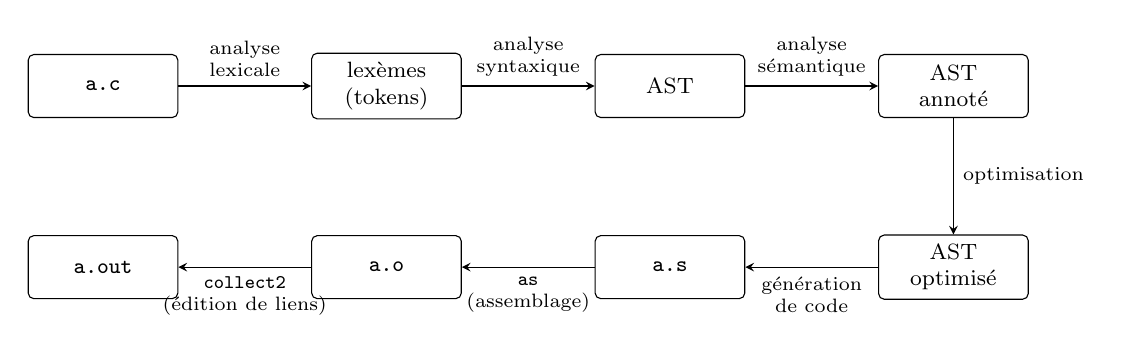
\begin{tikzpicture}[
      font=\footnotesize, >=stealth,
      box/.style={draw, rounded corners=2pt, minimum height=8mm,
                  minimum width=19mm, align=center},
      lab/.style={font=\scriptsize, align=center}
    ]
    \node[box] (c)   at (0,0)     {\texttt{a.c}};
    \node[box] (tok) at (3.6,0)   {lexèmes\\(tokens)};
    \node[box] (ast) at (7.2,0)   {AST};
    \node[box] (sem) at (10.8,0)  {AST\\annoté};
    \node[box] (opt) at (10.8,-2.3) {AST\\optimisé};
    \node[box] (asm) at (7.2,-2.3)  {\texttt{a.s}};
    \node[box] (obj) at (3.6,-2.3)  {\texttt{a.o}};
    \node[box] (bin) at (0,-2.3)    {\texttt{a.out}};
    \draw[->] (c)   -- node[lab,above]{analyse\\lexicale} (tok);
    \draw[->] (tok) -- node[lab,above]{analyse\\syntaxique} (ast);
    \draw[->] (ast) -- node[lab,above]{analyse\\sémantique} (sem);
    \draw[->] (sem) -- node[lab,right]{optimisation} (opt);
    \draw[->] (opt) -- node[lab,below]{génération\\de code} (asm);
    \draw[->] (asm) -- node[lab,below]{\texttt{as}\\(assemblage)} (obj);
    \draw[->] (obj) -- node[lab,below]{\texttt{collect2}\\(édition de liens)} (bin);
  \end{tikzpicture}
\end{figure}

The \textit{analysis} stages breaks up the source program into constituent
peices and imposes a grammatical structure on them. It then uses this structure
to create an intermediate representation of the source program. The
\textit{synthesis} stages construct the target program from the intermediate
representation and the information in the symbol table.

\subsection{Les étapes de l'analyse}
\subsubsection{Analyse Lexicale}
\begin{definition}[Analyse lexicale (\textit{lexing})]
  L'\textbf{analyse lexicale} a pour objectif de découper le fichier en une liste de
  lexèmes (\textit{tokens}); souvent à l'aide d'expressions régulières.
\end{definition}

The lexeur is the only stage that sees the file as a sequence of characters.
After it, whitespace, indentation and line breaks no longer exist.

\begin{example}[The token stream of \texttt{fibo}]
  The source on the left lexes to the stream on the right.
  \begin{multicols}{2}
    \begin{lstlisting}[language=C]
    int fibo(int n)
    {
      if(n<=1)
        return 1;
      return
         fibo(n-1)
       + fibo(n-2);
    }
    \end{lstlisting}
    \vfill\null
    \begin{lstlisting}
    INT ID("fibo") LPAR INT ID("n") RPAR
    LBRACKET
       IF LPAR ID("n") LEQ CST(1) RPAR
         RETURN CST(1) SEMICOL
       RETURN
        ID("fibo") LPAR ID("n") MINUS CST(1) RPAR
       PLUS
        ID("fibo") LPAR ID("n") MINUS CST(2) RPAR
       SEMICOL
    RBRACKET
    \end{lstlisting}
  \end{multicols}
\end{example}

\begin{remark}
This mapping into the token stream depends on the implementation and the
grammar of the source langauge, but each token usually carries an identifier
and a value.
\end{remark}

\subsubsection{Analyse Syntaxique}
\begin{definition}[Analyse syntaxique (\textit{parsing})]
  L'\textbf{analyse syntaxique} a pour objectif de récupérer la structure du
  code, généralement sous la forme d'un \textbf{arbre de syntaxe abstrait}
  (\textit{Abstract Syntax Tree}, AST) et souvent à l'aide d'une \textbf{grammaire}.
\end{definition}

\begin{example}[The AST of \texttt{fibo}]
  The token stream on the left parses to the AST on the right.
  \begin{multicols}{2}
    \begin{lstlisting}
    INT ID("fibo") LPAR INT ID("n") RPAR
    LBRACKET
       IF LPAR ID("n") LEQ CST(1) RPAR
         RETURN CST(1) SEMICOL
       RETURN
        ID("fibo") LPAR ID("n") MINUS CST(1) RPAR
       PLUS
        ID("fibo") LPAR ID("n") MINUS CST(2) RPAR
       SEMICOL
    RBRACKET
    \end{lstlisting}
    \vfill\null
    \begin{lstlisting}[language=Caml]
    Function( "fibo", [("n",Tint)],
       Sequence(
         If(Less(Var "n", Cst 1),
            Return (Cst 1)),
         Return Plus(
           Call("fibo",[Minus(Var "n", Cst 1)]),
           Call("fibo",[Minus(Var "n", Cst 2)])
          )
       )
    )
    \end{lstlisting}
  \end{multicols}
\end{example}
\begin{remark}
  The AST is only a common form of intermediate representation used by
  compilers. Alternatives include the \textit{three-address code} and the
  \textit{control-flow graph}.
\end{remark}

\subsubsection{Analyse Sémantique}
\begin{definition}[Analyse sémantique (\textit{semantic analysis})]
  L'\textbf{analyse sémantique} checks for semantic consistency with the
  language definition, and further gathers type information and saves it.
\end{definition}
This stage does not change the shape of the tree, only annotating it and
reject semantically inconsistent programs.
\begin{remark}
  Certain language specifications may permit type conversions known as
  \textit{coercions}, which typically overloads various operators and
  functions, and require conversion between types.
\end{remark}

\subsubsection{Optimisation}
\begin{definition}[Optimisation]
  L'\textbf{optimisation} a pour objectif de produire un code plus performant.
\end{definition}
An optimisation is a rewriting of the program which must preserve the
semantics; the analyses that justify the rewriting are what the names below
refer to.

\begin{example}[Élimination du code mort (\textit{dead code elimination})]
  The call under a condition that is statically false is removed.
\begin{lstlisting}[language=C]
int fibo(int n) {                         int fibo(int n) {
  if(n<=1)                                  if(n<=1)
    return 1;                                 return 1;
  if(false)                   ==>           return
    printf("fib %d\n",n);                     fibo(n-1)
  return                                    + fibo(n-2);
     fibo(n-1)                            }
   + fibo(n-2);
}
\end{lstlisting}
\end{example}

\begin{example}[Propagation des constantes (\textit{constant propagation})]
  A product of four \texttt{const int}s is evaluated at compile time.
\begin{lstlisting}[language=C]
const int days_in_year = 365 ;                const int days_in_year = 365 ;
const int hours_in_day = 24 ;                 const int hours_in_day = 24 ;
const int min_in_hours = 60 ;         ==>     const int min_in_hours = 60 ;
const int seconds_in_hours = 60 ;             const int seconds_in_hours = 60 ;
int main() {                                  int main() {
  printf("There are %d "                        printf("There are %d "
  "seconds in an ordinary year!",               "seconds in an ordinary year!",
  days_in_year * hours_in_day *                 31536000);
  min_in_hours * seconds_in_hours );          }
}
\end{lstlisting}
\end{example}

\begin{example}[Analyse des alias (\textit{alias analysis})]
  The load is replaced by the value that was just stored.
\begin{lstlisting}[language=C]
int f(int * a, int * b) {            int f(int * a, int * b) {
  *a = 42;                             *a = 42;
  *b = 12;                  ==>        *b = 12;
  return *a;                           return 42;
}                                    }
\end{lstlisting}
  This rewrite is legal exactly when the compiler can prove that \texttt{a} and \texttt{b} do not
\emph{alias}, i.e.\ do not point at the same cell.
\end{example}

Optimisation is non-trivial, often requiring global analyses of the program,
and is a major part of the work of a compiler. There are also other forms of
optimisations, such as dépliement de boucles (\textit{loop unrolling}), analyse
de vie (\textit{liveness analysis}), dead store, and sous-expressions communes
(\textit{common subexpression elimination}).

\subsection{Les étapes de la synthèse}
\subsubsection{Code Génération}
The first stage of \textit{synthesis} is code generation, which turns the intermediate
representation into the target language. In the context of \textit{code assembleur (x86)},
this produces a (still) human-readable text file of assembly instructions.

\begin{example}[\texttt{fibo} in x86-64 AT\&T assembly]
  What \texttt{cc1} emits for the source above.
\begin{lstlisting}[language=gas]
    .file    "a.c"
    .text
    .globl   fibo
    .type    fibo, @function
fibo:
.LFB0:
    .cfi_startproc
    pushq    %rbp
    .cfi_def_cfa_offset 16
    .cfi_offset 6, -16
    movq     %rsp, %rbp
    .cfi_def_cfa_register 6
    pushq    %rbx
    subq     $24, %rsp
    .cfi_offset 3, -24
\end{lstlisting}
$\qquad\quad\vdots$
\end{example}

\begin{remark}
  The lines beginning with a dot are \textbf{directives} addressed to the
  assembler, not instructions: \texttt{.text}, \texttt{.section .rodata},
  \texttt{.globl}, \texttt{.type} and \texttt{.size} organise the output. They
  produce no machine code.
\end{remark}

\subsubsection{Assemblage}
\begin{definition}[Assemblage]
  In the context of Linux / ELF, the assembleur turns that text into an fichier
  objet (\textit{object file}). The instructions are now octets, grouped into
  named sections.
\end{definition}

\begin{example}[A hex dump of \texttt{b.o}]
  What \texttt{as} emits, section by section.
\begin{lstlisting}
b.o:     file format elf64-x86-64

Contents of section .text:
 0000 554889e5 534883ec 18897dec 837dec01  UH..SH....}...}.
 0010 7f07b801 000000eb 1e8b45ec 83e80189  ..........E.....
 0020 c7e80000 000089c3 8b45ec83 e80289c7  .........E......
 0030 e8000000 0001d848 8b5df8c9 c3        .......H.].....
Contents of section .comment:
 0000 00474343 3a202844 65626961 6e203132  .GCC: (Debian 12
 0010 2e322e30 2d31342b 64656231 32753129  .2.0-14+deb12u1)
 0020 2031322e 322e3000                     12.2.0.
Contents of section .eh_frame:
 0000 14000000 00000000 017a5200 01781001  .........zR...x.
 0010 1b0c0708 90010000 1c000000 1c000000  ................
 0020 00000000 3d000000 00410e10 8602430d  ....=....A....C.
 0030 06458303 730c0708                    .E..s...
\end{lstlisting}
\end{example}

\subsubsection{Édition de liens}
\begin{definition}[Édition de liens (\textit{linking})]
  In Linux / ELF, the linker takes one or more object files and produces a
  single executable file. It resolves the references between the object files,
  and adds the C runtime startup code and the dynamic-linking machinery.
\end{definition}
This produce the fichier binaire (\textit{binary file}) that the operating
system can load and run.

\begin{example}[A word dump inside \texttt{a.out}]
  A window onto the symbol names the linker had to resolve.
\begin{lstlisting}
0000470 5f00 6c5f 6269 5f63 7473 7261 5f74 616d
0000480 6e69 5f00 635f 6178 665f 6e69 6c61 7a69
0000490 0065 7270 6e69 6674 6c00 6269 2e63 6f73
00004a0 362e 4700 494c 4342 325f 322e 352e 4700
00004b0 494c 4342 325f 332e 0034 495f 4d54 645f
00004c0 7265 6765 7369 6574 5472 434d 6f6c 656e
00004d0 6154 6c62 0065 5f5f 6d67 6e6f 735f 6174
00004e0 7472 5f5f 5f00 5449 5f4d 6572 6769 7374
00004f0 7265 4d54 6c43 6e6f 5465 6261 656c 0000
\end{lstlisting}
Each group is a 16-bit word printed in hexadecimal. On a petit-boutien machine,
we may recover the null-terminated strings by swapping each pair of two octets
and reading the result as ASCII:
\begin{lstlisting}
__libc_start_main   __cxa_finalize   printf   libc.so.6
GLIBC_2.2.5   GLIBC_2.34   _ITM_deregisterTMCloneTable
__gmon_start__   _ITM_registerTMCloneTable
\end{lstlisting}
\end{example}

\subsection{Le Pipeline de Compilation}
\begin{example}[Linux / ELF]
  Invoking \texttt{gcc a.c} triggers three tools in sequence:
  \begin{itemize}
    \item \verb|cc1 a.c a.s| --- produce the assembly from the C;
    \item \verb|as -o a.o a.s| --- produce the object from the assembly;
    \item \verb|collect2 a.o a.out| --- produce the binary from the object.
  \end{itemize}
  Each of these tools performs its own lexical, syntactic and semantic
  analyses. Additionally, each of the intermediate files can be inspected with
  the following commands:
  \begin{itemize}
    \item \texttt{gcc -S a.c} --- produce the assembly from the C;
    \item \texttt{as -o a.o a.s} --- produce the object from the assembly;
    \item \texttt{objdump -d a.o} --- produce a disassembly of the object;
    \item \texttt{objdump -d a.out} --- produce a disassembly of the binary.
  \end{itemize}
\end{example}

The compiler is a chain of programs, each potentially taken as compilers in
their own right, with its own input and output language.
